\chapter{Prediction System}
\label{PredictionSystem}
The main goal during this phase was to find a way to implement a forecast system in Python.
Since the datasets used during this thesis could be considered as a time series, it was decide to implement and test an Autoregressive Integrated Moving Average (ARIMA) model. \\
Since there are several possible configurations that fits an ARIMA model, it is important to find the right one to use with each input dataset because it would give much better prediction results.
In order to find the best ARIMA configuration there are different methods and procedures. The most known is "Box–Jenkins method"\footnote{Check out the Box–Jenkins method at the current link: \\ \url{https://en.wikipedia.org/wiki/Box\%E2\%80\%93Jenkins_method}}. In this study it was decided to use an easier method, in order to have a first approach with this system and a general idea about the problem. It basically consists of testing different ARIMA model configurations for the same input dataset and then comparing the results.\\
For this reason, during this phase of the work two different subsytems for two different purposes have been implemented:
\begin{enumerate}
\item Evaluating System
\item Prediction System
\end{enumerate}

\newpage
\section{Evaluating System}
\textbf{Goal:}\\ 
Used for evaluating different configurations of the ARIMA machine. \\ It tests 112 different configurations for the current input and reports the tested configurations with the corresponding MAPE (Mean Average Percentage Error)\footnote{MAPE formula and description: \\ \url{https://en.wikipedia.org/wiki/Mean_absolute_percentage_error}} value in a document. MAPE is a measure of prediction accuracy of a forecasting method in statistics, for example in trend estimation, and it usually expresses accuracy as a percentage.

\textbf{Requirements:}\\
There are not any kind of needed requirements. It's possible to use this system on dataset of arbitrary length.

\textbf{Code implementation:}\\
The most important part of the code about the Evaluating System is the following.\\
Basically the method ARIMA() allows to train a model based on historic values (history) and a specific order (p,d,q). After that it's possible to call the method forecast() through the trained model and having some predictions like result.
\begin{lstlisting}
model = ARIMA(history, order=arima_order)
model_fit = model.fit(disp=0)
yhat = model_fit.forecast()[0]
\end{lstlisting}

More specific, all the 112 different ARIMA configurations tested are all the possible combinations between the following three parameters values:
\begin{lstlisting}
p_values = [0, 1, 2, 4, 6, 8, 10]
d_values = [0, 1, 2, 3]
q_values = [0, 1, 2, 3]
\end{lstlisting}

It's important to remind that the following evaluation system is fitting the model with the first 66\% of the dataset values, and then the model forecasting is tested and compared on the final 34\% .\\

It's possible to check out the full implemented code in the appendice: [\ref{Evaluating_System}]

\newpage

\textbf{Results:}\\
The system will report the MAPE between real value and predicted values for each of the 112 tested ARIMA machine in a document.
During this part of the work also a script\footnote{Link to the implemented script "autoEvaluate.sh" : \\url{https://github.com/Sprea22/Personal\_Utilities}} for executing an ARIMA evaluation about each single parameter of each single dataset was created, but once executed it required too much time to complete all the evaluations.
For that reason, just some relevant evaluations result have been reported in a document. The table below reports some results about specific parameters that are going to be used in the next phase.\\

 \begin{table}[ht]
\makebox[\textwidth][c]{
    \begin{tabular}{ | l | l | l | l |}
            \hline
\textbf{Input} 	& \textbf{Parameter}	& \textbf{ARIMA Conf} 	& \textbf{MAPE result} 	\\ \hline
Finnmark & feedConsumption				& (6, 1, 0) 			& 13.771\% 		 		\\ \hline	
Hordaland & feedConsumption				& (8, 0, 0)  			& 6.811\%				\\ \hline				
Troms & feedConsumption					& (2, 0, 0)  			& 11.593\% 				\\ \hline
Nordland & feedConsumption				& (6, 0, 0)  			& 12.741\%		 	\\ \hline
Norway0714 & feedConsumption			& (6, 1, 0)  			& 7.296\%  				\\ \hline
    \end{tabular}}
         \caption{MAPE Results for some particular dataset about the parameter "feedConsumption"}   
   \label{table: MAPE_Results_feedConsumption} 
\end{table}     


 
\newpage
\section{Prediction System}
\textbf{Goal:}\\ 
This system has two main goals:
\vspace{-5mm}
\begin{itemize}
 \setlength{\itemsep}{-5pt} 
\item Predict some future value with the a specific ARIMA configuration.
\item Display the historic data together with real future values and predicted future values.
\end{itemize}

\textbf{Requirements:}\\
The only requirement is to use in a correct way this system is that the real future values are available, in order to compare it with the predicted one. It's possible to use this system on input dataset of arbitrary length.


\textbf{Code implementation:}\\
The method ARIMA() allows to train a model based on historic values (history) and a specific order (p,d,q). After that it's possible to call the method forecast() through the trained model with a "int" parameter that represents the desired number of predictions that have to be calculated.

\begin{lstlisting}
model = ARIMA(dataset, order=order)
model_fit = model.fit(disp=0)
forecast = model_fit.forecast(int(sys.argv[3]))[0]
\end{lstlisting}

Once calculated and saved the predictions in a document, the system will basically display on the same graphic "realVaues" that contains the real future values, "predFuture" that contains the predicted future values and "series" that contains the dataset historic values.
\begin{lstlisting}
ax.plot(realValues, "g", label='Real 2015 Values', linewidth=2)
ax.plot(predFuture, "r", label='Prediction 2015 values', linewidth=2)
ax.plot(series, "b", label='Historic values', linewidth=2)
\end{lstlisting}

It's possible to check out the full implemented code in the appendice: [\ref{Prediction_System}]

\newpage

\textbf{Results:}\\
This system will automatically generate a document that contain:
\vspace{-5mm}
\begin{itemize}
 \setlength{\itemsep}{-5pt} 
\item Real future values
\item Predicted future values
\item MAPE between each prediction and the corresponding real value.
\end{itemize}

It provides also the possibility to visualize the historic, real and predicted future values on the same graphic, as shown in the example figure [\ref{GraphicForecasting}].

\begin{figure}[H]
    \makebox[\textwidth][c]{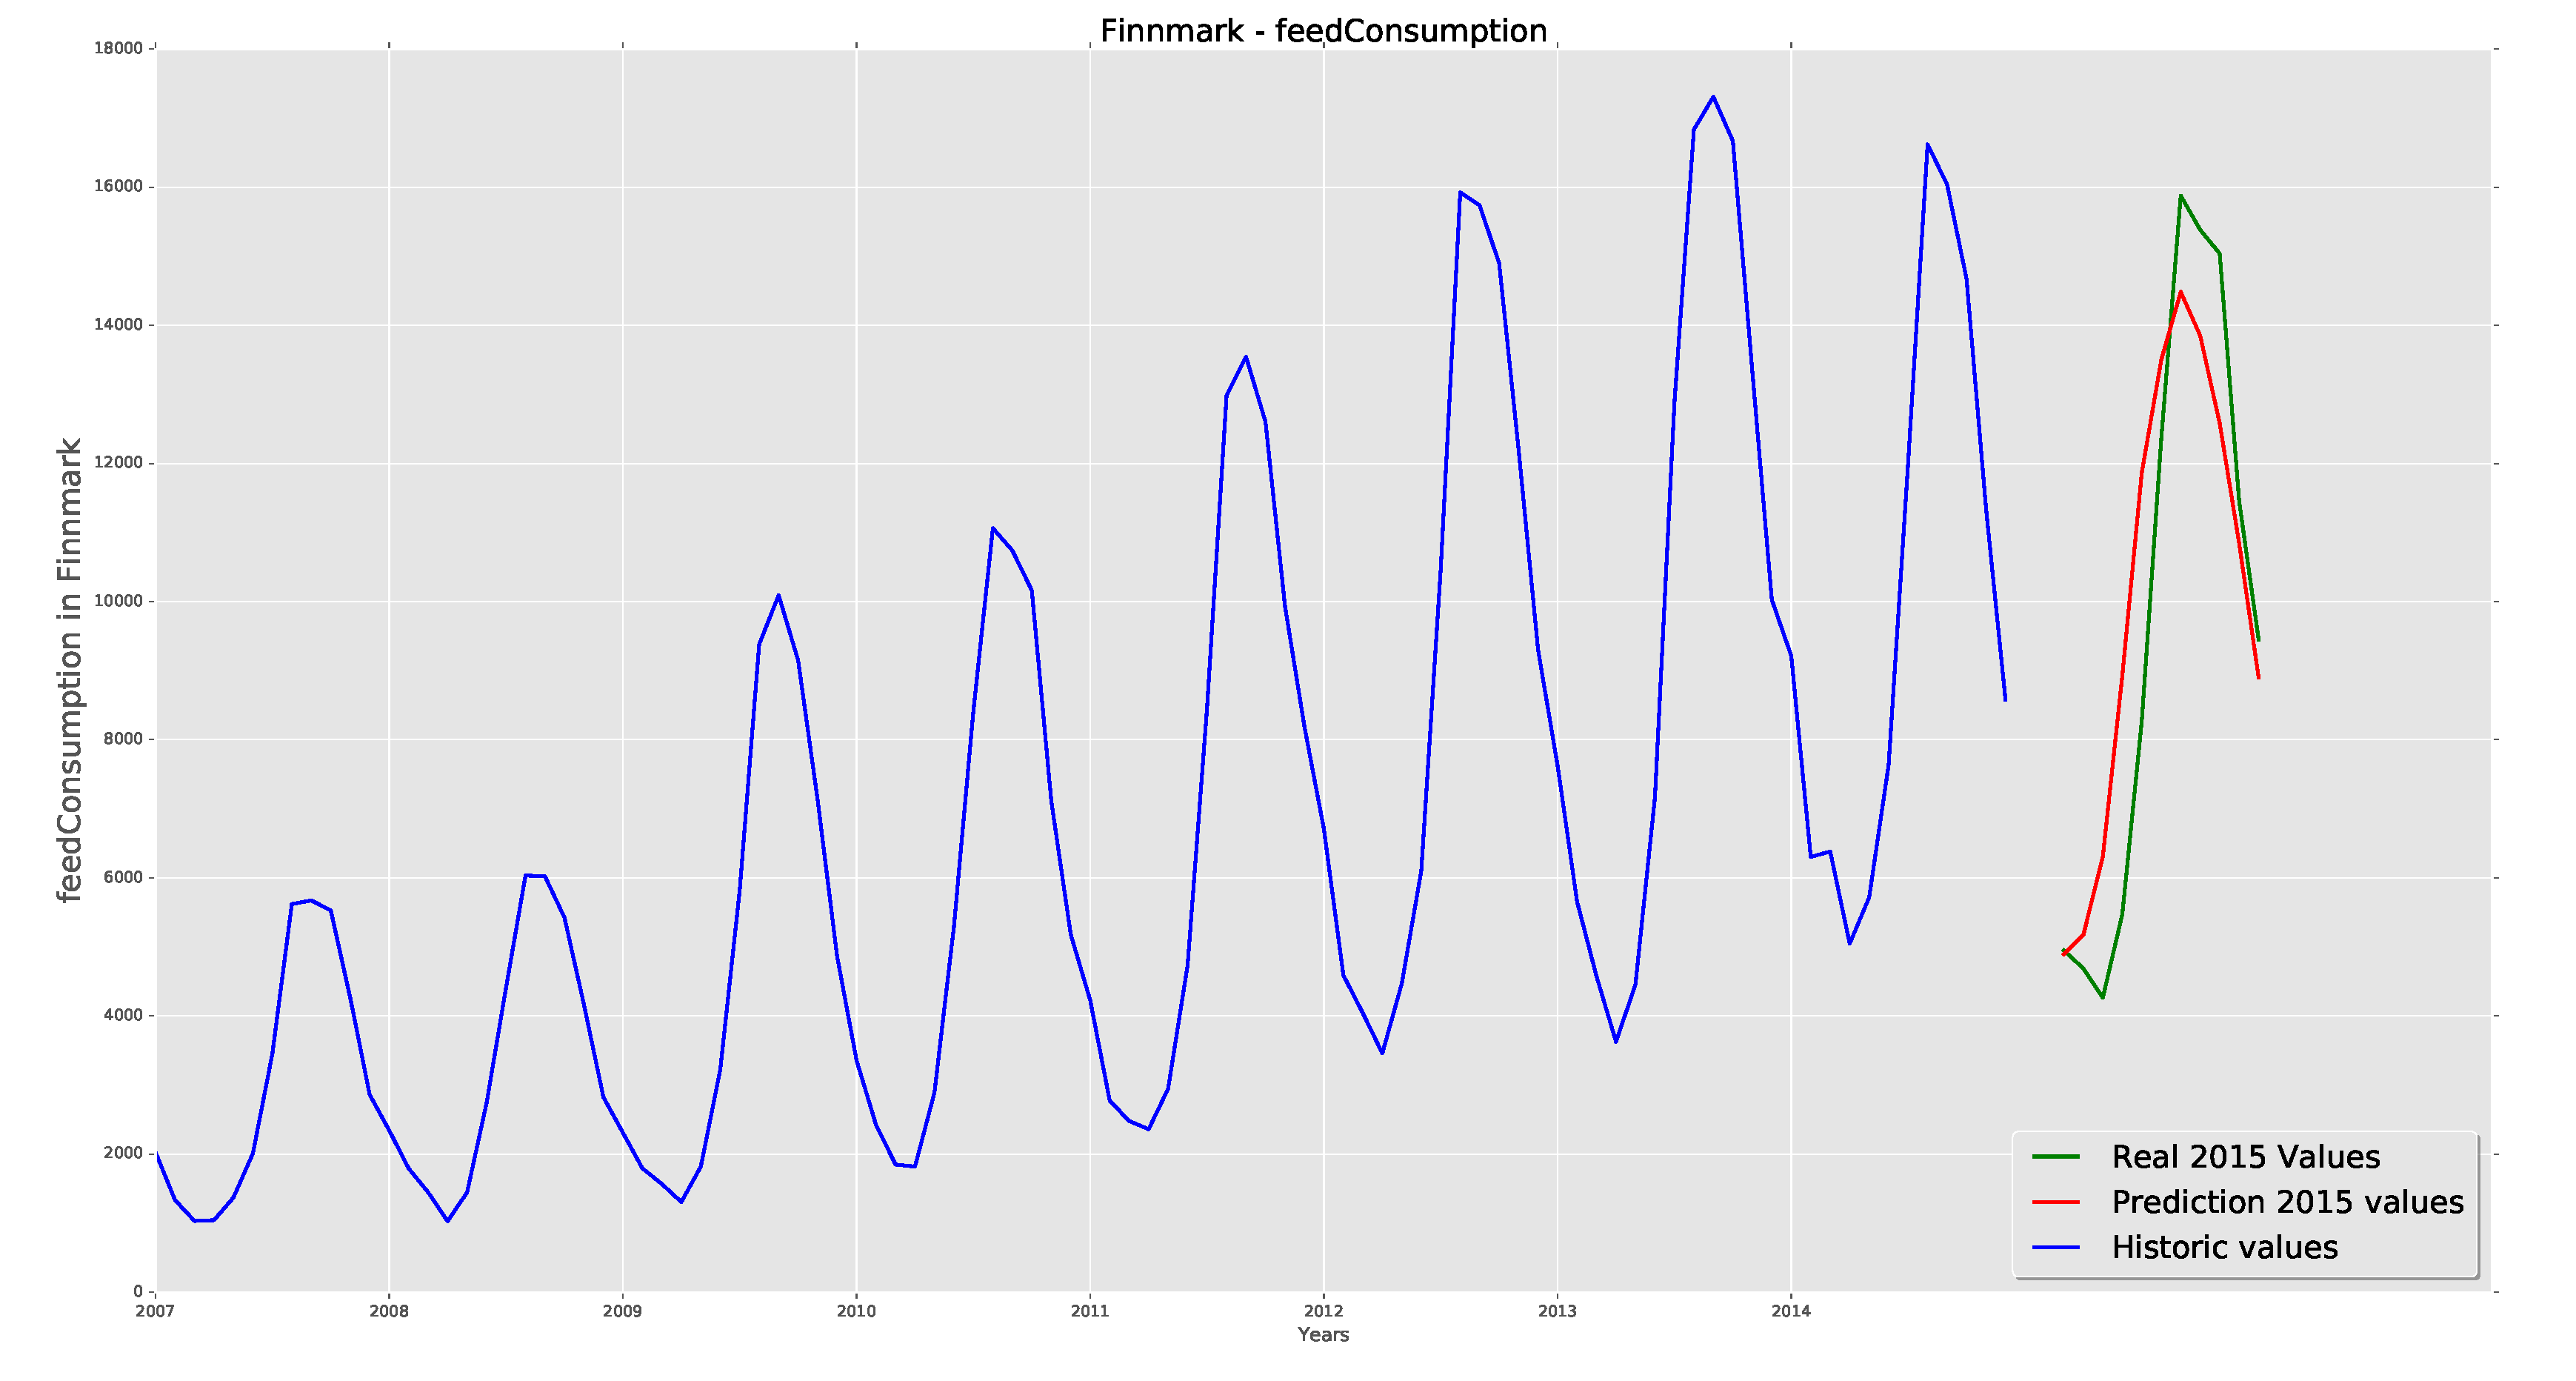
\includegraphics[width=1.3\textwidth]{Files/Finnmark-feedConsumption_pred.pdf}}
    \caption{Graphic that display historic, real and predicted future values of a input.}
\label{GraphicForecasting}
\end{figure}


\newpage



